%% Technical Report for the work on the AI-DSL over the period of May
%% to September 2022.

\documentclass[]{report}
\usepackage{url}
\usepackage{minted}
\usepackage[textsize=footnotesize]{todonotes}
\newcommand{\kabir}[2][]{\todo[color=yellow,author=kabir, #1]{#2}}
\newcommand{\nil}[2][]{\todo[color=purple,author=nil, #1]{#2}}
\usepackage[hyperindex,breaklinks]{hyperref}
\usepackage{breakurl}
\usepackage{listings}
\lstset{basicstyle=\ttfamily\footnotesize,breaklines=false,frame=single}
\usepackage{float}
\restylefloat{table}
\usepackage{longtable}
\usepackage{graphicx}
\usepackage[font=small,labelfont=bf]{caption}
\usepackage[skip=0pt]{subcaption}
\usepackage{circledsteps}

\begin{document}

\title{AI-DSL Technical Report (May to Septembre 2022)}
\author{Nil Geisweiller, Samuel Roberti}
\maketitle

\begin{abstract}
\end{abstract}

\tableofcontents

\chapter{Introduction}

\section{Setting the Scene}

In the previous iteration we explored using Dependent Types to express
formal specifications of AI services, with the ultimate goal of
building a language for easily writing those specifications, the
AI-DSL itself, as well as services to automatically connect AI
services together, the AI-DSL Registry~\cite{AIDSLReport2021}.

Back then we experimented with trivial AI services, computing simple
arithmetic, described by trivial properties, such as the parity of
their inputs/outputs.  We were able to demonstrate that Idris, our DTL
of choice, could be used to verify the correctness of such AI service
assemblages.  The approach seemed promising, but to really put the
idea to the test we had to make progress on two fronts:

\begin{enumerate}
\item Replace trivial AI services by actual AI algorithms.
\item Explore program synthesis, as it became clear that it was at the
  heart of this endeavor.  First, for building the AI service
  assemblages themselves.  Second, for achieving fuzzy matching, that
  is when AI services almost fit together but not quite yet.  And
  third, for completing assemblages when some AI services are outright
  missing.
\end{enumerate}
That is what we have done during that iteration.

\section{Work Accomplished}

First we have implemented three AI algorithms in Idris:
\begin{enumerate}
\item Gradient descent
\item Linear regression
\item Logistic regression
\end{enumerate}
These algorithms were chosen because they are relatively simple, yet
extensively use in real world applications, as well as tightly related
to each other.  Linear regression can be framed as a gradient descent
problem, and logistic regression can be framed both as gradient
descent and linear regression problems, thus constituting an excellent
case study for the AI-DSL.  Alongside these implementations, a
descending property was formulated and formally proved for each
algorithm.

Finally, we have explored ways to perform program synthesis of
dependently typed programs.  While we have only achieved partial
success as far as program synthesis is concerned, we were able to
demonstrate its feasibility within the Idris ecosystem.  It was clear
from the start anyway that to be done well and fully, program
synthesis essentially requires achieving AGI.  Indeed, it is one of
these AI-complete problems.  That is any problem can be framed as a
program synthesis problem and vice versa.  The idea being that such
functionality can be progressively grown, deferred less and less to
human intervention, as the network and the AI-DSL evolve.

\section{Related Work}

Here's a list of projects and publications we have discovered along
the way that relate to the work done during that iteration.  TODO

\chapter{Implementation and Verification of AI Algorithms}

\section{Implementation of AI Algorithms}
We have implemented the following AI algorithms in Idris:
\begin{enumerate}
\item Descent: a generic descending algorithm.
\item Gradient Descent: a gradient descent algorithm using Descent.
\item Linear Regression: a linear regression algorithm using Gradient
  Descent.
\item Logistic Regression: a logistic regression algorithm using
  Gradient Descent.
\item Logistic-Linear Regression: a logistic regression algorithm
  using Linear Regression.
\end{enumerate}
\begin{figure}[H]
  \centering
  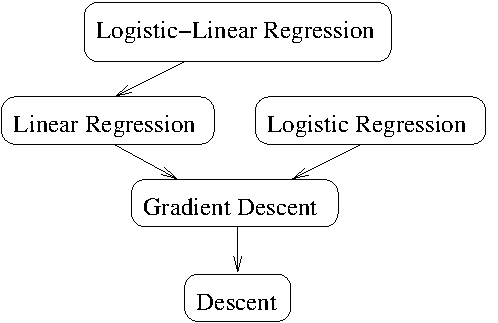
\includegraphics[scale=0.8]{figs/ai-algorithms.xfig.pdf}
  \caption{AI algorithms call graph}
  \label{fig:ai_algorithms}
\end{figure}
A call graph is provided in Figure~\ref{fig:ai_algorithms}.  Each
algorithm may be viewed as an AI service, together forming a network
of AI services delegating work to one another when possible.

The idea of performing logistic regression via two paths, either
directly via calling Gradient Descent, or indirectly via calling
Linear Regression, came from the ambitious goal of having our AI-DSL
prototype discover an alternate way, possibly unforeseen by the AI
practitioner, to perform a certain AI tasks, here logistic regression.
As we will see we did not come far enough to achieve that goal, but we
certainly keep on the side for the future.

Let us now describe in more details what these algorithms are doing,
and then provide the descending property we have focused on in this
work.

\subsection{Descent}
The Descent algorithm takes in input:
\begin{enumerate}
\item a cost function to minimize;
\item a step function to jump from candidate to candidate;
\item an initial candidate to start the search from;
\item a maximum number of steps allocated to the search;
\end{enumerate}
and outputs the final candidate as well as the remaining unallocated
steps.

\subsection{Gradient Descent}
The Gradient Descent algorithm takes in input:
\begin{enumerate}
\item a loss function;
\item a gradient function;
\item a learning rate, also called step size;
\item an initial candidate to start the search from;
\item a maximum number of steps allocated to the search;
\end{enumerate}
converts the gradient function and the learning rate into a step
function, calls the Descent algorithm and returns the final candidate
as well as the remaining unallocated steps.

\subsection{Linear Regression}
The Linear Regression algorithm takes in input:
\begin{enumerate}
\item a data set to explain, a matrix of inputs and a column vector
  of outputs;
\item a learning rate, also called step size;
\item an initial candidate to start the search from;
\item a maximum number of steps allocated to the search;
\end{enumerate}
defines a sum-of-squared-errors-based loss and gradient functions for
that data set, calls Gradient Descent and returns the final candidate
as well as the remaining unallocated steps.

\subsection{Logistic Regression}
The Logistic Regression algorithm takes in input:
\begin{enumerate}
\item a data set to explain, a matrix of inputs and a Boolean column
  vector of outputs;
\item a learning rate, also called step size;
\item an initial candidate to start the search from;
\item a maximum number of steps allocated to the search;
\end{enumerate}
defines a cross-entropy-based loss and gradient functions for that
data set, calls Gradient Descent and returns the final candidate as
well as the remaining unallocated steps.

\subsection{Logistic-Linear Regression}
The Logistic-Linear Regression algorithm takes in input:
\begin{enumerate}
\item a data set to explain, a Boolean matrix of inputs and a Boolean
  column vector of outputs;
\item a learning rate, also called step size;
\item an initial candidate to start the search from;
\item a maximum number of steps allocated to the search;
\end{enumerate}
transforms the data set so that the column vector of outputs
represents the odds of outputting True instead of a Boolean value,
calls linear regression on that transformed data set and returns the
final candidate as well as the remaining unallocated steps.

\section{Verification of AI Algorithms}

The concept of verifying properties of AI algorithms is a very broad
one, could be verifying the AI algorithms themselves, or their output
models, either using crisp mathematical properties, or empirical fuzzy
NEXT

Here we focus on the simplest one we could possibly come up with in
this situation, which is that the algorithm must descend, or at least
not ascend.  In other words, that the final candidate must be better,
or at least not worse, that the initial one.  This may seem like an
overly simplistic property, and it is.  However, as we will see,
working with that was already quite an educational journey.

Let us begin by showing the Idris implementation of Descent, or rather
a slightly simplified version modified for expository purpose:
\begin{minted}[mathescape]{idris}
descent : Ord cost_t =>
          (cnd_t -> cost_t) ->    -- Cost function
          (cnd_t -> cnd_t) ->     -- Step function
          (cnd_t, Nat) ->         -- Init candidate, steps
          (cnd_t, Nat)            -- Final candidate, steps
descent _ _ (cnd, Z) = (cnd, Z)
descent cost next (cnd, S k) = if cost (next cnd) < cost cnd
                               then descent cost next (next cnd, k)
                               else (cnd, (S k))
\end{minted}
It essentially expresses that if the cost of the next candidate is
less than the cost of the initial candidate, it should recursively
descend from the next candidate, otherwise return the initial
candidate.  The descending property can then be formalized as follows:
\begin{minted}[mathescape]{idris}
descent_le : Ord cost_t =>
             (cost : cnd_t -> cost_t) -> -- Cost function
             (next : cnd_t -> cnd_t) ->  -- Step function
             (cas : (cnd_t, Nat)) ->     -- Init candidate, steps
  (cost (fst (descent cost next cas)) <= cost (fst cas)) === True
\end{minted}
which expresses that the cost of the final candidate should be less
than or equal to the cost of the initial candidate\footnote{For
  information, \texttt{===} denotes the equality type, a dependent
  type with \texttt{Refl} as sole constructor corresponding to the
  reflexivity axiom of equality.}.  Obviously such property should be
trivial to proof given how the algorithm has been written.  In
practice however, it is not so trivial, for two reasons:
\begin{enumerate}
\item Idris makes no assumption about the comparison operators
  \texttt{<}, \texttt{>}, \texttt{<=} and \texttt{>=}.  The interface
  \texttt{Ord} guaranties that \texttt{cost\_t} implements these
  operators, but not how they should behave.  Thus one needs to encode
  these assumptions and make sure that they are true for the types of
  interest, which is not always easy, or even possible, especially for
  primitive types like \texttt{Double}.  NEXT: Stefane prim vs
  implementing ourselves.
\item As the algorithm is recursive, it requires a recursive proof.
\end{enumerate}
Here is a proof of \texttt{descent\_le}, slightly simplified as
\texttt{descent}.  Let us first deal with the case where the number of
allocated steps is zero:
\begin{minted}[mathescape]{idris}
descent_le _ _ (_, Z) = le_reflexive
\end{minted}
In order to proof the descending property it suffices to invoke the
reflexivity of \texttt{<=} since for that case \texttt{descent} merely
becomes the identity function.  Let us now examine the case where the
number of allocated steps is greater than zero:
\begin{minted}[mathescape]{idris}
descent_le cost next (cnd, S k)
           with ((cost (next cnd)) < (cost cnd)) proof eq
  _ | True = let des_le_nxtcst = descent_le cost next (next cnd, k)
                 nxtcst_le_cst = le_reflexive_closure_lt (Left eq)
              in le_transitive des_le_nxtcst nxtcst_le_cst
  _ | False = le_reflexive
\end{minted}
The proof considers the two branches of the conditional.  If the
condition is false then invoking the reflexivity of \texttt{<=}
suffices for the same reason as above.  If the condition is true then
the proof needs to combine more axioms pertaining to comparison with
the recursion of \texttt{descent\_le}.  That proof, even simplified,
is already somewhat substantial, likely too substantial to be rapidly
discovered by greedy proof search.  And the non simplified version,
which can be found here~\cite{TODO} is about twice that size.

NEXT: other algorithms.

\chapter{Program Synthesis}
\label{chap:program_synthesis}

\section{Language Framework}

\section{Idris Elaboration}

\section{Idris Proof Search}

Idris proof search, contrary to what its name may suggest, can be used
for program synthesis in general, not just proof search -- which is no
surprise to those familiar with the Curry-Howard correspondence.

\chapter{Conclusion}

\appendix
\chapter{Glossary}
\begin{itemize}
\item \textbf{AI service assemblage}: collection of AI services
  interacting together to fulfill a given function.  Example of such
  AI service assemblage would be the Nunet Fake News Warning system.
\item \textbf{Dependent Types}: types depending on values.  Instead of
  being limited to constants such as \texttt{Integer} or
  \texttt{String}, dependent types are essentially functions that take
  values and return types.  A dependent type is usually expressed as a
  term containing free variables.  An example of dependent type is
  \texttt{Vect n a}, representing the class of vectors containing
  \texttt{n} elements of type \texttt{a}.
\item \textbf{Dependently Typed Language}: functional programming
  language using dependent types.  Examples of such languages are
  Idris, AGDA and Coq.
\item \textbf{DTL}: Shorthand for Dependently Typed Language.
\end{itemize}

\bibliographystyle{splncs04}
\bibliography{local}

\end{document}
